\documentclass{cmspaper}
\usepackage{graphicx}
\usepackage{subfigure}
\usepackage{amsmath}
\usepackage{amssymb}
\usepackage[pdfborder=0 0 0,
            colorlinks,
            urlcolor = blue,
            linkcolor = black,
            citecolor = black,
            menucolor = black,]
           {hyperref}
%% \usepackage[colorlinks]{hyperref}
%% \usepackage{url}
\usepackage[toc,page]{appendix}
\renewcommand{\appendixname}{Appendix}
%% \renewcommand{\appendixtocname}{List of appendices}

\input{commands}
% useful definitions

% processes
\def\dyee {\ensuremath{Z/\gamma^*\to ee}}
\def\dymm {\ensuremath{Z/\gamma^*\to\mu\mu}}
\def\dytt {\ensuremath{Z/\gamma^*\to\tau\tau}}
\def\zee {\ensuremath{Z\to ee}}
\def\zmm {\ensuremath{Z\to\mu\mu}}
\def\ztt {\ensuremath{Z\to\tau\tau}}
\def\ttbar {\ensuremath{t\bar{t}}}
\def\wwll {\ensuremath{WW\to l^+l^-}}
\def\wwlulu{\ensuremath{WW\to l^+\nu l^-\bar{\nu}}}
\def\ww {\ensuremath{WW}}
\def\wz{\ensuremath{WZ}}
\def\zz{\ensuremath{ZZ}}
\def\wgamma{\ensuremath{W\gamma}}
\def\wjets{\ensuremath{W+}jets} 
\def\tw{\ensuremath{tW}} 
\def\singletopt{\ensuremath{t} ($t$-chan)} 
\def\singletops{\ensuremath{t} ($s$-chan)} 
\def\all{all}
\def\ee{\ensuremath{ee}}
\def\emu{\ensuremath{e\mu}}
\def\mm{\ensuremath{\mu\mu}}

%units

%others
\def\pt{\ensuremath{p_T}}
\def\ipb{pb\ensuremath{^{-1}}}
\def\ifb{fb\ensuremath{^{-1}}}
\def\et{\ensuremath{E_T}}
\def\met{\ensuremath{E\!\!\!\!/_T}}
\def\fBrem{\ensuremath{f_{\rm brem}}}
\def\pin{\ensuremath{p_{\rm in}}}
\def\pout{\ensuremath{p_{\rm out}}}


\setcounter{topnumber}{1}
\setcounter{bottomnumber}{1}

\begin{document}
\begin{titlepage}

  \analysisnote{2012/XXX}

  \date{\today}

  \title{Constraining Anomalous Triple Gauge Couplings in WW dilepton final state}
  
  \input{authors}

  \begin{abstract}
    This note describes the extraction of anomalous triple gauge
    couplings in the $WW$ di-lepton analysis using $\intlumi$ of data
    collected in the 2011 Run at $\sqrt{s} = $ 7~TeV center of mass
    energy. An unbinned maximum likelihood fit is used to fit for the
    leading lepton pt. At 95\% C.L. $\lambda_{Z}: [-0.04,0.04]$,
    $\Delta g^Z_1: [-0.07,0.07]$ and $\Delta\kappa_{\gamma}:
    [-0.18,0.14]$. The results are consistent with the Standard
    Model expectations.
  \end{abstract} 

\end{titlepage}
\tableofcontents
\listoftables
\listoffigures
\newpage 

\section{Introduction}
   \label{sec:introduction}
   Drell-Yan (\dyll) events represent the major background to a \hww~ signal in the same flavor final state.
After applying tight cuts on \met, they are highly suppressed but the expected signal yield is significantly 
reduced and the remaining \dyll~ background is difficult to estimate.
The net effect is that the sensitivity of the \hww~ analysis is dominated by the opposite flavor final state.

In the published 2011 analysis\cite{ref:hwwpaper}, the \dyll~ background is estimated using a method called \routin\cite{ref:hwwsmurfs}, 
which extrapolates to the signal region the \dyll~ yield in the $Z$ peak region. 
Results from the \routin method are generally stable but suffer from large statistical and systematic uncertainties.

In addition, the analysis relied on MC for deriving the shapes used in the BDT analysis; 
given that the Drell-Yan Monte Carlo sample with generator cut \mll$<$20 \GeVcc contained too few events and the statistical uncertainty 
in that region was too large, in the same flavor final state a \mll$>$ 20\GeVcc cut was applied and a significant fraction 
of a low-mass Higgs signal was lost.

The present note describes a new method for \dyll~estimation constituting a valid alternative 
to \routin, that can cross-check its results, provide shapes from data and possibly reduce the uncertainties.
The main idea is to use a ``fake-rate'' mathod, where the rate for \dyll\ events passing the final \met\ selection
is evaluated on a \gjets\ sample and applied to same flavor dilepton events in a loose \met\ region. 

\section{Data Samples}
  \label{sec:datasets}
  %UPDATEME%
The datasets used for this analysis are summarized in 
Tables~\ref{tab:DatasetsData} and~\ref{tab:DatasetsMC} for data and Monte 
Carlo, respectively. The total integrated luminosity is \intlumiEightTeV. 
We used the official good run list~\cite{json}. For Monte Carlo simulation 
we use madgraph when possible, but different generators such as Pythia and Powheg~\cite{powheg} 
are also used.  For $gg \to \WW$ a dedicated generator is used. For \wz\ and \zz\
processes we use Pythia, since MadGraph samples are mixed with $\WW$ in
a single $VV$ sample, which is difficult to use properly.

\begin{table}[!ht]
\begin{center}
\begin{tabular}{|c|c|}
\hline
 Dataset Description                   &   Dataset Name   \\
\hline \hline
\multirow{2}{*}{MuEl PromptReco}   		&  /MuEG/Run2012A-PromptReco-v1/AOD   \\
            							&  /MuEG/Run2012B-PromptReco-v1/AOD   \\
\multirow{2}{*}{DiMuon PromptReco}     	&  /DoubleMu/Run2012A-PromptReco-v1/AOD   \\
          								&  /DoubleMu/Run2012B-PromptReco-v1/AOD   \\
\multirow{2}{*}{DiElectron PromptReco} 	&  /DoubleElectron/Run2012A-PromptReco-v1/AOD   \\
      									&  /DoubleElectron/Run2012B-PromptReco-v1/AOD   \\
\multirow{2}{*}{SingleMuon PromptReco}  &  /SingleMu/Run2012A-PromptReco-v1/AOD   \\
      									&  /SingleMu/Run2012B-PromptReco-v1/AOD   \\
\multirow{2}{*}{SingleElectron PromptReco} 	&  /SingleElectron/Run2012A-PromptReco-v1/AOD   \\
      										&  /SingleElectron/Run2012B-PromptReco-v1/AOD   \\
\hline
\end{tabular}
\caption{Summary of data datasets used.\label{tab:DatasetsData}}
\end{center}
\end{table}

\begin{table}[!ht]
\begin{center}
{\footnotesize
\begin{tabular}{|c|c|c|}
\hline
\multicolumn{3}{|c|}{With Pileup: Processed dataset name is always} \\
\multicolumn{3}{|c|}{/Summer12-PU\_S7\_START52\_V9-v*/AODSIM} \\
\hline
 Dataset Description              		&   Primary Dataset Name   & cross-section (pb)\\
\hline
$\ttbar$                              	&   /TTJets\_TuneZ2star\_8TeV-madgraph-tauola                          	& 	225.2 	\\
tW                  	 	 			&   /T\_tW-channel-DR\_TuneZ2star\_8TeV-powheg-tauola                  	&  	11.18 	\\
$\bar{\textrm{t}}$W                   	&   /Tbar\_tW-channel-DR\_TuneZ2star\_8TeV-powheg-tauola               	&  	11.18 	\\
gg $\rightarrow WW \to 2l 2\nu$         &   /GluGluToWWTo4L\_TuneZ2star\_8TeV-gg2ww-pythia6                     &   1.74	\\
qq $\rightarrow WW$                  	&   /WWJetsTo2L2Nu\_TuneZ2star\_8TeV-madgraph-tauola                    &  	5.81  	\\
WZ                               	 	&   /WZ\_TuneZ2star\_8TeV\_pythia6\_tauola                        		&  	22.45 	\\
Z[10-50] 	  	 						&   /DYJetsToLL\_M-10To50filter\_8TeV-madgraph                   		&  	860.5 	\\
Z[50-inf] 	  	 						&   /DYJetsToLL\_M-50\_TuneZ2Star\_8TeV-madgraph-tarball           		&  	3532.8 	\\
ZZ $\rightarrow 2l 2\nu$    	 		& 	/ZZJetsTo2L2Nu\_TuneZ2star\_8TeV-madgraph-tauola                    &   0.365	\\
ZZ $\rightarrow 2l 2q$    	 			&   /ZZJetsTo2L2Q\_TuneZ2star\_8TeV-madgraph-tauola                     &   1.28	\\
ZZ $\rightarrow 4l$    	 				&   /ZZJetsTo4L\_TuneZ2star\_8TeV-madgraph-tauola                       &   0.0921	\\
$gg \to H \to WW \to 2l 2\nu$         	&   /GluGluToHToWWTo2LAndTau2Nu\_M-*\_8TeV-powheg-pythia6             	& 	vary 	\\
$qqH,~H \to WW \to 2l 2\nu$           	&   /VBF\_HToWWTo2LAndTau2Nu\_M-*\_8TeV-powheg-pythia6                 	& 	vary 	\\
$WH/ZH/\ttbar H,~H\to WW$              	&   /WH\_ZH\_TTH\_HToWW\_M-*\_8TeV-pythia6                            	& 	vary 	\\
\hline
\hline
\end{tabular}
}
\caption{Summary of Monte Carlo datasets used.\label{tab:DatasetsMC}. The cross sections for a SM Higgs boson
is taken from the LHC Higgs cross-section working group~\cite{LHCHiggsCrossSectionWorkingGroup:2011ti}}
\end{center}
\end{table}

Since some portion of data datasets were not processed, 
we use a json excluding missing events~\cite{json}. 
Last year we adjusted Higgs $\pt$ spectrum because 
the spectrum in the simulation (POWHEG 2.0) was harder than the one 
in the most precise calculation to NNLO with resummation to NNLL order.
In the new version of Powheg (POWHEG 2.1), this problem has been mostly resolved,
thus we do not apply any corrections for Higss $\pt$.

\section{Event Selection}
  \label{sec:selection}
  The fully leptonic final state consists of two isolated leptons
and large missing energy from the two undetectable neutrinos.
The major reducible background processes are \ttbar{}, \wjets{} and Drell-Yan. 
We thus perform several steps to select and extract the $\WW$ signal from data:

\begin{enumerate}
    \item We select events that pass pre-defined lepton triggers.
    \item We then select those events with two oppositely charged 
    high $\pt$ isolated leptons ($ee$, $\mu\mu$, $e\mu$) requiring:
        \begin{itemize}    
            \item $\pt>20~\GeVc$ for both leptons;
            \item standard identification and isolation requirements 
	    on both leptons.
        \end{itemize}
     \item We reject events with more than zero reconstructed jets;
     \item large transverse missing energy due to the neutrinos.
\end{enumerate}

The selection steps are now described in detail below.


\section{Method}
   \label{sec:method}
   \subsection{Method definition}

The basic idea of the \zm~method is to use a ``fake-rate'' method~\cite{fakeLeptonNote1,fakeLeptonNote2} based on \met.

Given a background process $B$ and a particular cut $c$ in the analysis suppressing $B$, a fake-rate method
estimates the yield of $B$ passing $c$ as the number of $B$ events failing $c$  
times a pass-to-fail ratio $R_{p-f}$
\begin{equation}
N_B\left(\mathrm{pass}\right)=N_B\left(\mathrm{fail}\right) \cdot R_{p-f}~,
\end{equation}
where $R_{pf}$ has to measured in an independent control sample 
reproducing with good accuracy the behavior of $B$ with respect to $c$.

Assuming that both in photon and \dyll~ events the sources of \met are the hadronic recoil against and pile-up effects, 
the \zm~method uses the \gjets~ sample to model the \met distribution in \dyll~events.
It defines a pass-to-fail ratio (\zm$\equiv$$R_{p-f}$) in bins of $N_{jets}$ and $p_{T}\left(\gamma\right)$:
\begin{equation}
\zeta\left(N_{jets},p_{T}\left(\gamma\right)\right)=\frac{N\left(N_{jets},p_{T}\left(\gamma\right), \met>\mwp\right)}{N\left(N_{jets},p_{T}\left(\gamma\right),\met<\mwp\right)}
\end{equation}
where $\mwp$ represents the working point chosen for the final \met~cut in the analyis.

In the same flavor dilepton sample, events passing the final analysis
selection but with $\met<\mwp$ are selected and \zm~is used to extrapolate to the signal region:
\begin{equation}
N_{\dyll}\left(\met>\mwp,N_{jets},p_{T}\left(\dil\right)\right)= \zeta\left(N_{jets},p_{T}\left(\dil\right)\right) \cdot N_{\dyll}\left(\met<\mwp,N_{jets},p_{T}\left(\dil\right)\right)
\end{equation}
where, in data, $N_{\dyll}\left(\met<\mwp\right)$ is computed subtracting opposite flavor and \V\Z~ events.

A corollary of the method is that shapes can be obtained from data by filling the histogram with \dyll~ events in the \met$<$\mwp~region 
with weight \zm~ (the same procedure is already used in 2011 analysis for the \Wjets~ background\cite{ref:shapenote}).

\subsection{The \hww~case}

In the \hww~analysis we consider events with dilepton $p_T$$>$45 \GeVc~and $\mathrm{min}$-$\mathrm{pmet}$$>$20 \GeV~ as a baseline common to same and opposite flavor final state~\cite{ref:hwwsmurfs};
$\mathrm{min}$-$\mathrm{pmet}$ is defined as:
\begin{equation}
\text{min-pmet} = \text{min(proj-pfMet,proj-trackMet)} ,
\end{equation}
where ``pfMet'' is the \met~reconstructed with the particle flow algorithm, ``trackMet'' is the \met~ constructed from charged particles consistent 
with originating from the primary vertex.
The ``proj-met'' variable (where met is either pfMet or trackMet) is defined as:
\begin{equation}
\text{proj-met} = 
\begin{cases} \met & \text{if $\Delta\phi_{min}>\frac{\pi}{2}$,}
\\
\met\sin(\Delta\phi_{min}) & \text{if $\Delta\phi_{min}<\frac{\pi}{2}$}
\end{cases}
\end{equation}
\begin{equation}
\text{with } \Delta\phi_{min} =  min(\Delta\phi(\ell_1,\met),\Delta\phi(\ell_2,\met))\\
\end{equation}
where $\Delta\phi(\ell_i,\met)$ is the angle between \met\ and lepton $i$ in the transverse plane;
the main purpose for using ``proj-met'' is to reduce the impact of lepton mismeasurement and, secondarily, to further suppress the contribution from \dytt.
The final \met~ selection in the same flavor dilepton final state requires min-pmet$>$(37+nvtx/2) \GeV. 

In the photon sample this selection is reproduced by cutting on min-met=$\mathrm{min(pfMet,trackMet)}$ and photon $p_T$.
In photon events, ``proj-met'' variables cannot be defined because is not possible to project on lepton directions, so the \zm~ method will not 
predict the contribution from fake \met~due to lepton mismesurement. 
However, as it shown in Figures \ref{fig:met_0j}-\ref{fig:met_1j}, despite the slightly different definiton, the photon sample reproduces with 
good precision the \met in the \dyll~sample.

Is summary, we use the following definitions:
\begin{itemize}
\item dilepton sample pass region: min-pmet$>$(37+nvtx/2) \GeV, dilepton $p_T$$>$45 \GeVc
\item dilepton sample fail region: 20$<$min-pmet$<$(37+nvtx/2) \GeV, dilepton $p_T$$>$45 \GeVc
\item photon sample pass region: min-met$>$(37+nvtx/2) \GeV, photon $p_T$$>$45 \GeVc
\item photon sample fail region: 20$<$min-met$<$(37+nvtx/2) \GeV, photon $p_T$$>$45 \GeVc
\end{itemize}

%%%%%%%%
\begin{figure}[!hbtp]
\begin{center}
\subfigure[proj-pfMet in \dyll~ sample]{\label{subfig:pmet_0j}
\includegraphics[width=.4\textwidth]{figures/pmet_0j.png}}
\subfigure[pfMet in \gjets~ sample]{\label{subfig:met_0j}
\includegraphics[width=.4\textwidth]{figures/met_0j.png}}\\
\subfigure[proj-trackMet in \dyll~ sample]{\label{subfig:pTrackMet_0j}
\includegraphics[width=.4\textwidth]{figures/pTrackMet_0j.png}}
\subfigure[trackMet in \gjets~ sample]{\label{subfig:trackMet_0j}
\includegraphics[width=.4\textwidth]{figures/trackMet_0j.png}}
\caption{\met in the 0-jet bin. 
For visualization purposes, the \gjets~ and \dyll~contributions from MC are scaled by a had-hoc scale factor to macth data in the bulk of the distribution.
In the \gjets~ sample, data is shown after re-weighting to the \dyll~$p_T$ distribution in MC events.}
\label{fig:met_0j}
\end{center}
\end{figure}
%%%%%%%%

%%%%%%%%
\begin{figure}[!hbtp]
\begin{center}
\subfigure[proj-pfMet in \dyll~ sample]{\label{subfig:pmet_1j}
\includegraphics[width=.4\textwidth]{figures/pmet_1j.png}}
\subfigure[pfMet in \gjets~ sample]{\label{subfig:met_1j}
\includegraphics[width=.4\textwidth]{figures/met_1j.png}}\\
\subfigure[proj-trackMet in \dyll~ sample]{\label{subfig:pTrackMet_1j}
\includegraphics[width=.4\textwidth]{figures/pTrackMet_1j.png}}
\subfigure[trackMet in \gjets~ sample]{\label{subfig:trackMet_1j}
\includegraphics[width=.4\textwidth]{figures/trackMet_1j.png}}
\caption{\met in the 1-jet bin. 
For visualization purposes, the \gjets~ and \dyll~contributions from MC are scaled by a had-hoc scale factor to macth data in the bulk of the distribution.
In the \gjets~ sample, data is shown after re-weighting to the \dyll~$p_T$ distribution in MC events.}
\label{fig:met_1j}
\end{center}
\end{figure}
%%%%%%%%

%%%%%%%%
\begin{figure}[!hbtp]
\begin{center}
\subfigure[proj-pfMet in \dyll~ sample]{\label{subfig:pmet_2j}
\includegraphics[width=.4\textwidth]{figures/pmet_2j.png}}
\subfigure[pfMet in \gjets~ sample]{\label{subfig:met_2j}
\includegraphics[width=.4\textwidth]{figures/met_2j.png}}\\
\subfigure[proj-trackMet in \dyll~ sample]{\label{subfig:pTrackMet_2j}
\includegraphics[width=.4\textwidth]{figures/pTrackMet_2j.png}}
\subfigure[trackMet in \gjets~ sample]{\label{subfig:trackMet_2j}
\includegraphics[width=.4\textwidth]{figures/trackMet_2j.png}}
\caption{\met in the 2-jet bin. 
For visualization purposes, the \gjets~ and \dyll~contributions from MC are scaled by a had-hoc scale factor to macth data in the bulk of the distribution.
In the \gjets~ sample, data is shown after re-weighting to the \dyll~$p_T$ distribution in MC events.}
\label{fig:met_2j}
\end{center}
\end{figure}
%%%%%%%%

\clearpage

\subsection{Evaluation of \zm}

For each jet bin, \zm~ is evaluated both on MC and data samples in bins of photon $p_T$.
In data, the expected backgrounds with non-fake \met~ are subtracted from the photon sample.
Results for WW level in  are shown in Figures~\ref{fig:zeta_MC} and~\ref{fig:zeta_mh0}.
These are the values used for the \hww~ BDT shape analysis.

In the cut based analysis, an additional narrow cut on the transverse Higgs mass is applied~\cite{ref:hwwsmurfs}, where the following definition of $m_T$ is used:
\begin{equation}
m_{T} = \sqrt{2\pt^{ll}\met(1-cos(\Delta\phi_{\ell\ell-\met}))}
\end{equation}
where $\Delta\phi_{\ell\ell-\met}$ is the angle between dilepton direction and \met\ in the transverse plane.
For example, in the \mHi=120 \GeVcc~ analysis the signal region requires 70$<$$m_T$$<$120 \GeVcc.
Given that \met\ and $m_T$ are correlated variables, the \zm\ value depends on the $m_T$ cut value; 
therefore, \zm\ is derived separately for each Higgs mass analysis applying the corresponding $m_T$ cut on the photon sample.

A few representative results for \zm~derived from data for Higgs level cut based analysis are shown in Figures~\ref{fig:zeta_mh120}-\ref{fig:zeta_mh160}.

%%%%%%%%
\begin{figure}[!hbtp]
\begin{center}
\subfigure[0-jet]{\label{subfig:zeta_MC_0j_minmet}
\includegraphics[width=.4\textwidth]{figures/zeta_MC_0j_minmet.png}}
\subfigure[1-jet]{\label{subfig:zeta_MC_1j_minmet}
\includegraphics[width=.4\textwidth]{figures/zeta_MC_1j_minmet.png}}\\
\subfigure[2-jet]{\label{subfig:zeta_MC_2j_minmet}
\includegraphics[width=.4\textwidth]{figures/zeta_MC_2j_minmet.png}}
\caption{\zm~in MC at \WW~level.}
\label{fig:zeta_MC}
\end{center}
\end{figure}
%%%%%%%%

%%%%%%%%
\begin{figure}[!hbtp]
\begin{center}
\subfigure[0-jet]{\label{subfig:zeta_mass0_0j_minmet}
\includegraphics[width=.4\textwidth]{figures/zeta_mass0_0j_minmet.png}}
\subfigure[1-jet]{\label{subfig:zeta_mass0_1j_minmet}
\includegraphics[width=.4\textwidth]{figures/zeta_mass0_1j_minmet.png}}\\
\subfigure[2-jet]{\label{subfig:zeta_mass0_2j_minmet}
\includegraphics[width=.4\textwidth]{figures/zeta_mass0_2j_minmet.png}}
\caption{\zm~in data at \WW~level.}
\label{fig:zeta_mh0}
\end{center}
\end{figure}
%%%%%%%%

%%%%%%%%
\begin{figure}[!hbtp]
\begin{center}
\subfigure[0-jet]{\label{subfig:zeta_mass120_0j_minmet}
\includegraphics[width=.4\textwidth]{figures/zeta_mass120_0j_minmet.png}}
\subfigure[1-jet]{\label{subfig:zeta_mass120_1j_minmet}
\includegraphics[width=.4\textwidth]{figures/zeta_mass120_1j_minmet.png}}\\
\subfigure[2-jet]{\label{subfig:zeta_mass120_2j_minmet}
\includegraphics[width=.4\textwidth]{figures/zeta_mass120_2j_minmet.png}}
\caption{\zm~in data for \mHi=120 \GeVcc.}
\label{fig:zeta_mh120}
\end{center}
\end{figure}
%%%%%%%%

%%%%%%%%
\begin{figure}[!hbtp]
\begin{center}
\subfigure[0-jet]{\label{subfig:zeta_mass140_0j_minmet}
\includegraphics[width=.4\textwidth]{figures/zeta_mass140_0j_minmet.png}}
\subfigure[1-jet]{\label{subfig:zeta_mass140_1j_minmet}
\includegraphics[width=.4\textwidth]{figures/zeta_mass140_1j_minmet.png}}\\
\subfigure[2-jet]{\label{subfig:zeta_mass140_2j_minmet}
\includegraphics[width=.4\textwidth]{figures/zeta_mass140_2j_minmet.png}}
\caption{\zm~in data for \mHi=140 \GeVcc.}
\label{fig:zeta_mh140}
\end{center}
\end{figure}
%%%%%%%%

%%%%%%%%
\begin{figure}[!hbtp]
\begin{center}
\subfigure[0-jet]{\label{subfig:zeta_mass160_0j_minmet}
\includegraphics[width=.4\textwidth]{figures/zeta_mass160_0j_minmet.png}}
\subfigure[1-jet]{\label{subfig:zeta_mass160_1j_minmet}
\includegraphics[width=.4\textwidth]{figures/zeta_mass160_1j_minmet.png}}\\
\subfigure[2-jet]{\label{subfig:zeta_mass160_2j_minmet}
\includegraphics[width=.4\textwidth]{figures/zeta_mass160_2j_minmet.png}}
\caption{\zm~in data for \mHi=160 \GeVcc.}
\label{fig:zeta_mh160}
\end{center}
\end{figure}
%%%%%%%%

\clearpage

\section{Existing limits}
   \label{sec:limits}
   \fixme{Make sure it's all up to date}

The current best fit results for anomalous couplings are dominated by LEP
results. Table~\ref{tab:limits} shows the existing limits for various
couplings~\cite{ref:atgc_d0,ref:pdg}

\begin{table}[htp]
\caption[Current limits on anomalous couplings] {Current limits on
  anomalous couplings. The world best limits are based on a fit of LEP
  measurements. Tevatron results are shown for comparison. }
\begin{center}
\begin{tabular}{|c|c|}
\hline
 Coupling & Particle Data Group Fit \\
\hline
$\Lambda_\gamma$      & $-0.028^{+0.020}_{-0.021}$ \\
$\Lambda_Z$           & $-0.088^{+0.060}_{-0.057}$ \\
$\Delta g^Z_1$        & $-0.016^{+0.022}_{-0.019}$ \\
$\Delta\kappa_\gamma$ & $-0.027^{+0.044}_{-0.045}$ \\
$\Delta\kappa_Z$      & $-0.026^{+0.059}_{-0.056}$ \\
\hline
\end{tabular}
\begin{tabular}{|c|c|c|}
\hline
 Coupling & Tevatron ($\ww+\wz\to\ell\nu2\mathrm{jet}$) & Tevatron (\wwlulu{}) \\
\hline
$\Lambda=\Lambda_\gamma=\Lambda_Z$      & [-0.10,0.11] at 95\% C.L. & [-0.14,0.18] at 95\% C.L. \\
$\Delta\kappa_\gamma$                   & [-0.44,0.55] at 95\% C.L. & [-0.54,0.83] at 95\% C.L. \\
$\Delta g^Z_1$                          & [-0.12,0.20] at 95\% C.L. & [-0.14,0.30] at 95\% C.L. \\
\hline
\end{tabular}
\end{center}
\label{tab:limits}
\end{table}

\section{Monte Carlo modeling of anomalous couplings}
   \label{sec:modeling}
   We use MCFM NLO generator to produce the leading lepton \pt\
distributions for a number of points with non-zero anomalous
couplings. The distributions are corrected for the acceptance and
lepton reconstruction efficiency derived from a fully simulated Monte
Carlo sample. The Standard Model distribution has very few events for
large values of the leading lepton pt. It is hard to get large enough
sample of events generated with MCFM to cover this region. Therefore
we rely on the nominal Madgraph WW Monte Carlo to get the leading
lepton \pt\ distribution for the case of zero anomalous couplings. A
comparison of the distributions from different generators can be seen
in Figure~\ref{fig:generator_comparison}. It shows a good agreement
between Madgraph and MCFM distribtions.

\begin{figure}[tp]
  \centerline{
    \includegraphics[width=0.6\textwidth]{figures/generator_comparison.pdf}
%    \includegraphics[width=0.45\textwidth]{figures/generator_comparison_atgc.pdf}
  }

  \caption[Generator comparison]{Leading lepton \pt\ distribution
  for \WW\ simulated data using Madgraph (full simulation), MC@NLO (full simulation),
  Sherpa (fast simulation) and MCFM (reweighted). No aTGC.}

  \label{fig:generator_comparison}
\end{figure}

It is important to confirm that all the distributions are consistent
with the model used to parametrize the leading lepton \pt\ for
arbitrary couplings. Figure~\ref{fig:pdfs} shows the result of the signal PDF
parameterization using non-parametric PDFs based on histograms. It
reveals good agreement between the initial PDFs from the
generated samples and the final aTGC model.

\begin{figure}[tp]
  \centerline{
    \includegraphics[width=1.0\textwidth]{figures/pdfs}
  }

  \caption[PDF parameterization] {Leading lepton \pt\ distributions
  for \ww\ events with and without aTGCs. The black points represent the
  true \pt\ distribution for Monte Carlo events that passed the final
  selection. The blue dots show the \pt\ distribution from the model used to
  parametrize the anomalous coupling effects across different values
  of the couplings.}
\label{fig:pdfs}
\end{figure}


\clearpage
\section{Standard Model \ww\ yields}
   \label{sec:smww}
   
Table~\ref{tab:bkg_estimation} summarizes the estimation of background
yields using primarily data driven methods as described in Ref. \cite{ref:WWXS2011}.

\begin{table}[!ht]
  \begin{center}
 {\small
  \begin{tabular} {|c|c|c|c|c|c|c|}
\hline
      &   data & all bkg. & $qq \to \WW$ & $gg \to \WW$ &  $\ttbar+tW$   & $\Wjets$    \\
\hline
\hline
 $ee+\mu\mu$    &  462 & 94.8 $\pm$  4.4 & 296.8 $\pm$  2.7 & 17.7 $\pm$  0.4 & 43.8 $\pm$  1.3 & 15.9 $\pm$  2.3 \\ 
 $e\mu + \mu e$ &  668 & 146.4 $\pm$  4.8 & 477.2 $\pm$  3.4 & 28.2 $\pm$  0.5 & 77.8 $\pm$  1.8 & 42.4 $\pm$  3.2 \\ 
 Total & 1130   & 241.1 $\pm$  6.5 & 774.0 $\pm$  4.4 & 45.9 $\pm$  0.6 & 121.6 $\pm$  2.2 & 58.3 $\pm$  3.9 \\ 
 \hline
  \end{tabular}
  }

 {\small
  \begin{tabular} {|c|c|c|c|c|}
 \hline
   & $WZ$/$ZZ$ & $\dyll$ & $W+\gamma$ & \dytt \\
\hline
\hline
 $ee+\mu\mu$    & 18.1 $\pm$  0.4 & 11.7 $\pm$  3.2 &  5.3 $\pm$  1.4 &  0.0 $\pm$  0.0 \\ 
 $e\mu + \mu e$ & 11.0 $\pm$  0.2 &  0.0 $\pm$  0.0 & 14.5 $\pm$  3.1 &  0.8 $\pm$  0.2 \\ 
 Total          & 29.1 $\pm$  0.4 & 11.7 $\pm$  3.2 & 19.8 $\pm$  3.4 &  0.8 $\pm$  0.2 \\ 
\hline
  \end{tabular}
  }
  \caption{Expected number of signal and background events for an
  integrated luminosity of \intlumi, together with the data event yields, after
  applying the full selection. Monte Carlo statistical uncertainties are
  included.}
   \label{tab:bkg_estimation}
  \end{center}
\end{table}


\section{Fit validation}
   \label{sec:validation}
   The validation of the maximum likelihood fit, used to extract all information in this
analysis, is now described. The validation procedure consists of
two main tests. The first test is a fit using a data sample without
anomalous couplings. Such a test allows to identify problems with
event generation causing discrepancies in the leading lepton
\pt\ distribution. The second test is a fit using a data sample with
anomalous couplings. Such a test checks if we can properly measure
anomalous couplings when they are present. Both tests are critical to
validate the fitting tools, which are fairly complicated.

In the previous analysis it was found that the leading lepton
\pt\ distribution does not allow to differentiate between different
couplings and a typical observation inconsistent with Standard Model
represents a class of possible coupling values.

Figure~\ref{fig:val_scans} shows fit results and likelihood scans for
\ww\ simulated data with and without anomalous couplings. One may
conclude that even though the fit was able to measure the couplings
close to the true values, there is large uncertainty on the angle
between the two couplings as is revealed in the shapes of the contour
plots in the likelihood scans.

\begin{figure}[tp]
  \centerline{
    \includegraphics[width=1.0\textwidth]{figures/validation_likelihood_scans}
  }

  \caption[Likelihood scan for Signal Monte Carlo] {Likelihood scans
    for 350/pb of data excluding backgrounds. The curves
    represent the $\sqrt{2\Delta\log L}$ 1D significance of the difference between the
    likelihood with the sample's true anomalous couplings and the other
    values on the plain. The black star is the fit result when both couplings are
    allowed to float in the fit. The black point is the true value of the couplings.}
  \label{fig:val_scans}
\end{figure}

\subsection{Pseudo-experiments}
Figures~\ref{fig:fit_ww_mc_1D} and \ref{fig:fit_wwATGC_mc_1D_abs} show
results of the fits on \ww\ Monte Carlo samples with and without
anomalous couplings and excluding backgrounds. If only one coupling is
fitted it is not possible to get the sign right, so only absolute
values can be measured.

Pseudo-experiments with Standard Model \ww\ Monte Carlo are performed to look
for bias in the fit for the central value and to test the uncertainty
estimation. No significant deviation from zero is
found. Pseudo-experiments with non-zero anomalous couplings underestimate 
the true value by 20-30\%. To take this effect into
account we rescale final results.

\begin{figure}[tp]
  \centering
    \includegraphics[width=1.0\textwidth]{figures/fit_ww_mc_1D}
    \includegraphics[width=1.0\textwidth]{figures/fit_ww_mc_1D_2}

  \caption[1D fits to WW SM Monte Carlo] {Fit results for
  2-dimentional $\lambda_{Z}$-$\Delta g^Z_1$ (top) and
  $\lambda_{Z}$-$\Delta\kappa_\gamma$ (bottom) aTGC models using 50
  independent pseudo-data experiments made of Madgraph Standard
  Model \ww\ simulated data. Only one coupling floating in the fit,
  while the other one is fixed to the Standard Model
  value. Backgrounds are excluded from the fits.}

\label{fig:fit_ww_mc_1D}
\end{figure}


%% \begin{figure}[tp]
%%   \centerline{
%%     \includegraphics[width=1.0\textwidth]{figures/fit_wwATGC_mc_1D_pm}
%%   }

%%   \caption[1D fits to WW aTGC Monte Carlo] {Fits to WW Monte Carlo
%%     samples with anomalous couplings with 11 events in a sample. No
%%     background. Only one coupling is floated in the fit. Sign of the
%%     coupling cannot be determined in the fit.}
%%   \label{fig:fit_wwATGC_mc_1D_pm}
%% \end{figure}

\begin{figure}[tp]
  \centering
    \includegraphics[width=0.8\textwidth]{figures/fit_wwATGC_mc_1D_abs}
    \includegraphics[width=0.8\textwidth]{figures/fit_wwATGC_mc_1D_abs2}

  \caption[1D fits to WW aTGC Monte Carlo] {Fits to $WW$ Monte Carlo
    samples with anomalous couplings. Pseudo-data experiments are made
    with 5-10 times lower number of events in each experiment due
    limited amount of simulated data. Backgrounds are excluded from
    the fits. Only one coupling is allowed to float in the
    fit. Absolute values of the couplings are  shown.}  
    \label{fig:fit_wwATGC_mc_1D_abs}
\end{figure}

\subsection{Fit on data}
We check how much the normalization of different components were
changed during the fit with respect to the inial values. For this test
we treat anomalous couplings as nuisance parameters and hide their
central values.

Table~\ref{tab:fit_yields} summarizes the fit results for event
yields. From it we conclude that the excess of the events that we
observed in the cross-section measurement is absorbed mostly in \ww\
event yield. Looking at the correlation matrix
Figure~\ref{fig:fit_correlations} one can see that there is
significant correlation between \ww{}, \wjets{} and \ttbar{} event
yields. Figure~\ref{fig:fit_data} shows a reasonable agreement of the
final fit pt distribution and the one observed in data. 

%% Minuit2Minimizer: Minimize with max iterations 4000 edmval 1 strategy 1
%% Minuit2Minimizer : Valid minimum - status = 0
%% FVAL  = -1578.2051799912831
%% Edm   = 2.84316661007704903e-06
%% Nfcn  = 177
%% n_dy	  = 14.2216	 +/-  6.60059	(limited)
%% n_top	  = 88.7706	 +/-  21.5922	(limited)
%% n_wjets	  = 86.5649	 +/-  19.9815	(limited)
%% n_ww	  = 915.148	 +/-  45.4547	(limited)
%% n_wz	  = 18.5309	 +/-  1.89849	(limited)
%% n_zz	  = 10.5487	 +/-  0.999248	(limited)
%% x_par	  = 0.00401641	 +/-  0.0229406	(limited)
%% y_par	  = 0.00828161	 +/-  0.0352541	(limited)
%% Minos: Lower error for parameter 0  :  -6.73027
%% Minos: Upper error for parameter 0  :  6.74416
%% Minos: Lower error for parameter 1  :  -21.6282
%% Minos: Upper error for parameter 1  :  21.6914
%% Minos: Lower error for parameter 2  :  -20.078
%% Minos: Upper error for parameter 2  :  20.0657
%% Minos: Lower error for parameter 3  :  -45.2995
%% Minos: Upper error for parameter 3  :  45.6166
%% Minos: Lower error for parameter 4  :  -1.9004
%% Minos: Upper error for parameter 4  :  1.89958
%% Minos: Lower error for parameter 5  :  -1.00008
%% Minos: Upper error for parameter 5  :  0.999759
%% Minos: Lower error for parameter 6  :  -0.0227218
%% Minos: Upper error for parameter 6  :  0.020276
%% Minos: Lower error for parameter 7  :  -0.0348234
%% Minos: Upper error for parameter 7  :  0.0323726


\begin{table}[!ht]
  \begin{center}
 {\small
  \begin{tabular} {|l|c|c|c|}
\hline
  Parameter       &   Initial value & Fit value & Global Correlation \\
\hline
  N$_{\ww}$       & $819.9\pm57.6$  & $915.1\pm45.5$ & 0.69 \\
  N$_{Top}$       & $121.6\pm23.4$  & $88.8\pm21.6$  & 0.52 \\
  N$_{\wjets}$    & $78.1\pm22.0$   & $86.6\pm20.0$ & 0.55 \\
  N$_{\wz}$       & $18.5\pm1.9$    & $18.5\pm1.9$   & 0.06 \\
  N$_{\dyll}$     & $11.7\pm6.8$    & $14.2\pm6.6$   & 0.22 \\
  N$_{\zz}$       & $10.6\pm1.0$    & $10.5\pm1.0$   & 0.03 \\
\hline
  \end{tabular}
  }
  \caption{Nominal fit parameter values.}
   \label{tab:fit_yields}
  \end{center}
\end{table}

\begin{figure}[tp]
  \centering
    \includegraphics[width=.60\textwidth]{figures/correlations}

  \caption[Fit parameter correlations] {Correlation matrix for the nominal fit parameters.}
  \label{fig:fit_correlations}
\end{figure}

\begin{figure}[tp]
  \centering
    \includegraphics[width=.45\textwidth]{figures/lz_dgz_pdf_data}
    \includegraphics[width=.45\textwidth]{figures/lz_dkg_pdf_data}

  \caption[Fit on data] {Final combined pdf distribution (blue
  histogram) on top of observed data yield. Left plot shows results
  for a fit using $\lambda_Z$-$\Delta g^Z_1$ model and the right one
  shows that of $\lambda_Z$-$\Delta\kappa_{\gamma}$ model.} \label{fig:fit_data}
\end{figure}

\clearpage
\section{Results}
   \label{sec:results}
   

\begin{figure}[!htbp]
\begin{center}
   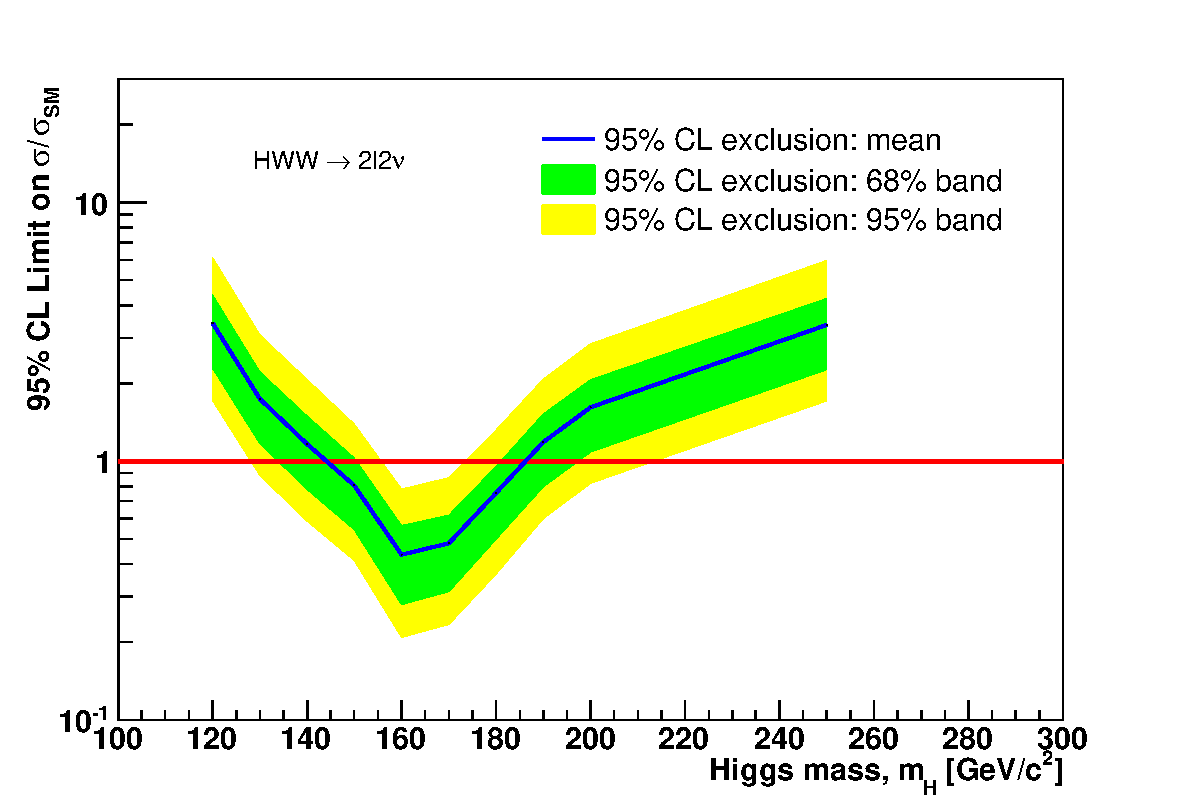
\includegraphics[width=0.9\textwidth]{figures/cut_based_limits.pdf}
   \caption{Cut based analysis expected upper limits at 95\%C.L. for 1\ifb\ of data.}
   \label{fig:cutbase_uls}
\end{center}
\end{figure}

\section{Conclusion}
   The \zm\ and \routin\ methods for DY estimation provide compatible results both in terms of DY estimation and in terms of final limits.
In 2012 analysis, the two methods will cross-check each other and the one with lowest uncertainty will be used as default method.

\clearpage
\clearpage

\vspace*{-0.2cm}
\thebibliography{12}

\bibitem{pdg}
 K. Nakamura et al. (Particle Data Group), "Review of particle physics", J. Phys.G37 , 2010.

\bibitem{Higgs1}
F. Englert and R. Brout, "Broken symmetries and the masses of gauge bosons", Phys. Rev. Lett. 13,  1964.

\bibitem{Higgs2}
P. W. Higgs, "Broken symmetry and the mass of gauge vector mesons", Phys. Rev. Lett. 13, 1964.

\bibitem{Higgs3}
Guralnik, G.S. and Hagen, C.R. and Kibble, T.W.B., "Global Conservation Laws and Massless Particles", 
Phys.Rev.Lett. 13, 1964.

\bibitem{HWW2010}
CMS Collaboration, "Title: Measurement of WW Production and Search for the Higgs Boson in 
pp Collisions at $\sqrt{s}$ = 7 TeV", arXiv:1102.5429

\bibitem{VBTFCrossSectionNote}
J. Alcaraz Maestre, \textit{et al.}, "Updated Measurements of Inclusive W and Z Cross Sections 
at $\sqrt{s}=7$ TeV", CMS AN-2010/264.

\bibitem{ggWWError}
F.~ Stoeckli, "http://indico.cern.ch/getFile.py/access?contribId=0\&resId=1\&materialId=slides\&confId=49009", 
EWK Diboson meeting of March 12 2009.

\bibitem{json}
{\small
/afs/cern.ch/cms/CAF/CMSCOMM/COMM\_DQM/certification/Collisions11/7TeV/Prompt/Cert\_160404-163869\_7TeV\_PromptReco\_Collisions11\_JSON.txt
}

\bibitem{ElIso}
A. Vartak, M. LeBourgeois, V. Sharma, "Lepton Isolation in the CMS Tracker, ECAL and HCAL", CMS AN-2010/106.

\bibitem{PVDA}
W. Erdmann, M. LeBourgeois, B. Mangano, 
https://indico.cern.ch/getFile.py/access?contribId=5\&sessionId=3\&resId=1\&materialId=slides\&confId=127127, 
note in preparation.

\bibitem{NExpHits}
B. Mangano \textit{et al.}, "Improvement in Photon Conversion Rejection Performance Using 
Advanced Tracking Tools", AN-10-283.

\bibitem{fakeLeptonNote1}
S.~Xie, \textit{et al.}", "Study of Data-Driven Methods for Estimation of Fake Lepton Backgrounds", 
CMS AN-2009/120.

\bibitem{fakeLeptonNote2}
W.~Andrews, \textit{et al.}, "Fake Rates for dilepton Analyses", CMS AN-2010/257.

\bibitem{fakeLeptonBkgSpillage1}
 F. Golf, D. Evans, J. Mulmenstadt  \textit{et al.}, ``Expectations for observation of top quark pair production in the dilepton final state with the early CMS data'', CMS AN-2009/050.

\bibitem{dyestnote}
W. Andrews, et al., “A Method to Measure the Contribution of $\dyll$ to a di-lepton+ MET Selection”, CMS AN-2009/023 (2009).

\bibitem{jes}
CMS Collaboration, "Jet Energy Calibration with Photon+Jet Events", PAS JME-09-004.

\bibitem{jetpas}
CMS Collaboration, "Jet Performance in pp Collisions at $\sqrt{s}=7 \rm\ TeV$", PAS JME-10-003.

\bibitem{btag}
CMS collaboration, "Commissioning of b-jet identification with pp collisions at $\sqrt{s}=7~\TeV$, BTV-10-001.

\bibitem{antikt}
Cacciari, Matteo and Salam, Gavin P. and Soyez, Gregory, "The anti-$k_t$ jet clustering 
algorithm", JHEP 04,  2008.

\bibitem{ConversionNote}
W.~Andrews, \textit{et al.}, "Study of photon conversion rejection at CMS", CMS AN-2009/159.

\bibitem{tmva}
A. Hoecker, \textit{et al.}, "TMVA - Toolkit for Multivariate Data Analysis", arXiv:physics/0703039, 2007.

\bibitem{XS}
CMS Generator group, Standard Model Cross Sections for CMS at 7 TeV, 2010.

\bibitem{PDF4LHC}
PDF4LHC Working Group, 
{\tt http://www.hep.ucl.ac.uk/pdf4lhc/PDF4LHCrecom.pdf}

\bibitem{Nadolsky:2008zw}
Nadolsky, Pavel M. and others, "Implications of CTEQ global analysis for 
collider observables", Phys. Rev. D78 2008.

\bibitem{Martin:2009iq}
Martin, A. D. and Stirling, W. J. and Thorne, R. S. and Watt, G., "Parton 
distributions for the LHC, Eur. Phys. J. C63 2009.

\bibitem{Ball:2010de}
Ball, Richard D. and others, "A first unbiased global NLO determination 
of parton distributions and their uncertainties", arXiv 1002.4407.

\bibitem{bayesian}
A. O'Hagan and J.J. Forster, "Bayesian Inference", Kendall's Advanced Theory of Statistics, 
Arnold, London, 2B, 2004.

\bibitem{ref:tagprobe_mit_w}
G. Bauer {\it et. al.}, "Lepton ef?iencies for the inclusive W cross section measurement with 36.1pb$^{-1}$", AN2011/097

\bibitem{ref:tagprobe_snt_top}
W. Andrews {\it et. al.}, "Uncertainties on the Lepton Selection Efficiency for t$t\bar{t}$ Cross Section Analysis", AN2010/274

\bibitem{LHCHiggsCrossSectionWorkingGroup:2011ti}
LHC Higgs Cross Section Working Group, "Handbook of LHC Higgs Cross Sections: 
Inclusive Observables", CERN-2011-002, 2011.

\bibitem{PFMET} 
CMS Collaboration, ``CMS MET Performance in Events Containing Electroweak Bosons from pp Collisions at $\sqrt{s}=7$ TeV'', CMS PAS JME-2010-005 (2010)


\bibitem{trkMET} 
Marco Zanetti, ``MET with PU in $\hww\to2\ell$'', https://indico.cern.ch/conferenceDisplay.py?confId=131580
Benjamin Hooberman, ``MET with PU in MC and First 2011 Data'', https://indico.cern.ch/contributionDisplay.py?contribId=5\&confId=132579. 


\bibitem{lands}
Mingshui Chen and Andrey Korytov, https://mschen.web.cern.ch/mschen/lands/

\bibitem{MCFMHiggsProduction}
J. Campbell, R.K. Ellis, G. Zanderighi, ``Next-to-Leading order Higgs + 2 jet production via gluon fusion.'', JHEP 0610:028 (2006), hep-ph/0608194
\clearpage
\appendix
\section{Limits using CLs method}
   We considered an alternative approach for setting the upper limits on
aTGC using the $CL_{s}$ method. Due to complexity of the method we had
to rely on existing tools in the Higgs group. In order to minimize
amount of work needed, we adopted a binned-likelihood appoach that may
lead to slightly different results.

The likelihood function is defined as:
\begin{eqnarray}
  L(\rm{data}|\mu,\theta)&=&\rm{Poisson}(\rm{data}|\mu\cdot s(\theta)+b(\theta))\cdot p(\tilde{\theta}|\theta) \nonumber\\
 &=&\prod_i\frac{(\mu s_i+b_i)^{n_i}}{n_i!}e^{-\mu s_i-b_i}\cdot p(\tilde{\theta}|\theta)
\label{eq:likelihood}
\end{eqnarray}
where $\mu$ is the signal strength modifier which is often reported in
the upper limit results as a ratio of the cross-section upper limit
over the standard model cross-section and $\theta$ represents a full
set of nuisance parameters that are used to incorporate systematic
uncertainties. 

As it was described earlier, the model used to parameterize aTGC
provides the leading lepton \pt\ distribution of the \ww\ system as a
function of the anomalous couplings. To extract CLs limits we had to
explicitely separate the Standard Model and anomalous parts of the
distribution. The effect of anomalous couplings on the leading
lepton \pt\ can lead to lower differential cross-section at low \pt\
values. In these cases we set the expected cross-section to be
zero. This should not have significant impact on results, since aTGC
mostly enter as events with \pt{}.

For $CL_{s}$ method the test statistic is defined as a likelihood
ratio:
\begin{equation}
\tilde{q_\mu}=-2\log\frac{L(\rm{data}|\mu,\hat\theta_\mu)}{L(\rm{data}|\hat\mu,\hat\theta)}
\end{equation}
where the numerator corresponds to the maximum likelihood for given
``data'' and $\mu$ profiling over the nuisance parameters and the
denominator corresponds to the maximum likelihood for given ``data''
profiling over the nuisance parameters and $\mu$. This test statistic
differs from the ones used at LEP (no profiling of systematic errors)
and at Tevatron (the denominator likelihood uses $\mu=0$ and only
systematic errors are profiled).

Figure~\ref{fig:cls} show the upper limit for one
and two dimentional models. The limits are found to be:
\begin{align}
  \lambda_{Z}: [-0.05,0.046]~95\%~\mathrm{C.L.}\\ 
  \Delta g^{Z}_1: [-0.084,0.07]~95\%~\mathrm{C.L.}\\
\end{align}
The results are consistent with the profiled-likelihood method. It is
important to take into account that we used the asymptotic $CL_{s}$
method, which relies on the linear behaviour of the likelihood to get
the expected limits correctly. It was found that limits extracted in
the profiled-likelihood method using explicit scan of the likelihood
(Minos) were different (smaller) than those derived using an
extrapolation (Migrad/Hesse). Producing ``full'' $CL_{s}$ limits would
take a lot of time and it is not justified for a cross-check. Without
such test the coverage of the $1\sigma$ and $2\sigma$ bands is not
guaranteed.

\begin{figure}[!hbtp]
\centering
\includegraphics[width=.45\textwidth]{figures/lz_cls.pdf}
\includegraphics[width=.45\textwidth]{figures/dgz_cls.pdf}
\includegraphics[width=.45\textwidth]{figures/lz_dgz_cls.pdf}
\caption{One and two dimensional $CL_{s}$ upper limits.}
\label{fig:cls}
\end{figure}

\end{document}
